
%(BEGIN_QUESTION)
% Copyright 2015, Tony R. Kuphaldt, released under the Creative Commons Attribution License (v 1.0)
% This means you may do almost anything with this work of mine, so long as you give me proper credit

Denne produksjonsprosessen produserer {\it ammoniumnitrat}, en hovedbestanddel i kunstgjødsel, ved kjemisk kombinasjon av salpetersyre og ammoniakk:

$$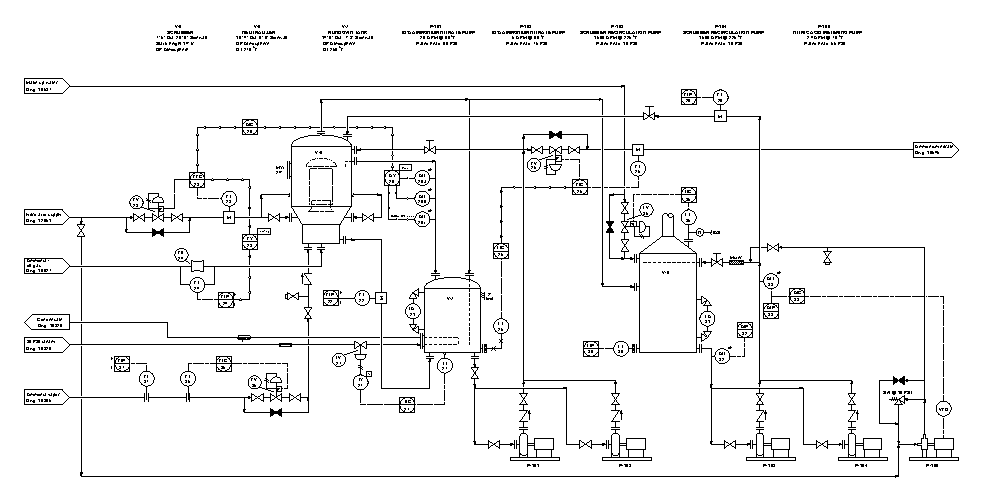
\includegraphics[width=15.5cm]{i0008rx01.eps}$$

Undersøk nivåreguleringssystemet for scrubber-beholderen (V-5). Anta at du får opplyst at forsyningstrykket i påfyllsvann-headeren har betydelige variasjoner, og at dette opptrer som en last i nivåreguleringssløyfen til V-5. Forklar hvordan du kan legge til kaskaderegulering i denne nivåsløyfen for bedre å håndtere svingninger i påfyllsvannets forsyningstrykk.

\underbar{file i01277}
%(END_QUESTION)





%(BEGIN_ANSWER)

Kaskaderegulering fungerer ved å legge til en ekstra regulator foran sluttelementet, som tar setpunktordre fra den opprinnelige sløyferegulatoren for å sikre at den manipulerte variabelen holder seg på denne verdien. I denne anvendelsen styrer nivåregulator LIC-35 ventilen LV-35 direkte for å slippe inn påfyllsvann til scrubberen etter behov for å holde nivået konstant i scrubberen. Vannforsyningstrykket er en last for nivåreguleringen fordi endringer i vannforsyningstrykket vil påvirke flowen inn i V-5 direkte for en gitt ventilstilling, noe som tvinger nivåregulator LIC-35 til å kompensere når den ser at væskenivået driver bort fra setpunktet.

\vskip 10pt

For å legge til kaskaderegulering i denne anvendelsen må vi først legge til en flowmåler i påfyllsvannlinjen slik at vi kan overvåke vannflowen inn i V-5. Deretter legger vi til en flowregulator (FIC) i sløyfen, som måler flow fra den nye transmitteren og bruker utgangen fra LIC-35 som fjernsetpunkt. Reguleringsventilen (LV-35) vil nå styres av utgangen fra flowregulatoren i stedet for utgangen fra nivåregulatoren.
 
\vskip 10pt

Forutsatt signal-til-åpne-virkning for LV-35 må den nye flowregulatoren konfigureres med {\it revers virkning} (dvs. den skal kommandere LV-35 mot lukket hvis flow overstiger setpunktet gitt av LIC-35).

%(END_ANSWER)





%(BEGIN_NOTES)


%INDEX% Control, strategies: cascade
%INDEX% Process: ammonium nitrate production (realistic P&ID shown)

%(END_NOTES)

